% This is a self-contained tex taken from USENIX style latex template. 

\documentclass[letter,twocolumn,10pt]{article}
\usepackage[margin=1in]{geometry}
\usepackage{enumitem}
\usepackage{url}
\usepackage{makecell}
\usepackage{csquotes}
\usepackage{booktabs}
\usepackage{tabularx}
\usepackage{tikz}
\usepackage{amsmath}
\usepackage{graphicx}
\usepackage{subcaption}
\usepackage[numbers,sort&compress]{natbib}
\usepackage[super]{nth}
\usepackage{breakurl}
\usepackage[breaklinks]{hyperref}
\def\UrlBreaks{\do\/\do-}

\setlength{\textheight}{9.0in}
\setlength{\columnsep}{0.33in}
\setlength{\textwidth}{7.00in}
\setlength{\topmargin}{0.0in}
\setlength{\headheight}{0.0in}
\setlength{\headsep}{0.0in}
\addtolength{\oddsidemargin}{-0.25in}
\addtolength{\evensidemargin}{-0.25in}

\def\@maketitle{\newpage
 \vbox to 2.5in{
 \vspace*{\fill}
 \vskip 2em
 \begin{center}%
  {\Large\bf \@title \par}%
  \vskip 0.375in minus 0.300in
  {\large\it
   \lineskip .5em
   \begin{tabular}[t]{c}\@author
   \end{tabular}\par}%
 \end{center}%
 \par
 \vspace*{\fill}
 }
}

\begin{filecontents}{\jobname.bib}
@Book{arpaciDusseau18:osbook,
  author =       {Arpaci-Dusseau, Remzi H. and Arpaci-Dusseau Andrea C.},
  title =        {Operating Systems: Three Easy Pieces},
  publisher =    {Arpaci-Dusseau Books, LLC},
  year =         2015,
  edition =      {1.00},
  note =         {\url{http://pages.cs.wisc.edu/~remzi/OSTEP/}}
}
@InProceedings{waldspurger02,
  author =       {Waldspurger, Carl A.},
  title =        {Memory resource management in {VMware ESX} server},
  booktitle =    {USENIX Symposium on Operating System Design and
                  Implementation (OSDI)},
  year =         2002,
  pages =        {181--194},
  note =         {\url{https://www.usenix.org/legacy/event/osdi02/tech/waldspurger/waldspurger.pdf}}
}
@inproceedings{CooperSTRS10socc,
  author    = {Brian F. Cooper and
               Adam Silberstein and
               Erwin Tam and
               Raghu Ramakrishnan and
               Russell Sears},
  title     = {Benchmarking cloud serving systems with {YCSB}},
  booktitle = {Proceedings of the 1st {ACM} Symposium on Cloud Computing, SoCC 2010,
               Indianapolis, Indiana, USA, June 10-11, 2010},
  pages     = {143--154},
  year      = {2010},
  doi       = {10.1145/1807128.1807152}
}
@misc{leveldb,
    author={Google},
    title={LevelDB},
    howpublished={\url{https://github.com/google/leveldb}}
}
@misc{rocksdb,
    author={Facebook},
    title={RocksDB},
    howpublished={\url{https://github.com/facebook/rocksdb}}
}

\end{filecontents}

\begin{document}

\date{}

%-------------------------------------------------------------------------------
%TODO You should come up with a compelling title. 
\title{\Large \textbf{Project 1 Report}}
%TODO Your name. 
\author{Kai Li}
%-------------------------------------------------------------------------------
\maketitle

%-------------------------------------------------------------------------------
\section*{Abstract}
%-------------------------------------------------------------------------------
LevelDB has been a very popular key-store in the Database systems. In this project, we demo how to build LevelDB from source and run some benchmarks to show the performance on our own computer. We further tune some configurable parameters and explain how each of them affects the system's performance through experiments.
%-------------------------------------------------------------------------------
\section{Introduction}
%-------------------------------------------------------------------------------
In order to understand the properties of LevelDB~\cite{leveldb} and how each configureable knobs influence the performance, a scientific methods is to instrument it and conduct experiments to obtain the first-hand experience. First of all, we need to clone the source code from Github ~\cite{XXX} and build the binaries from the source code. By following the README file, you are supposed to build the binaries, as well as some built-in benchmark tools such as \textsf{db\_bench}, \textsf{skiplist\_test} and so on. Once you build everything correctly, you can locate the binaries in the build folder, as shown by ~\ref{Fig}. The next step naturally is to run some banchmark binaries to get a sense of how the output format looks like, in my case, I executed two of them, db_bench and XXX, the results are shown by ~\ref{XXX} and ~\ref{XXX} respectively. There are other benchmarks (e.g.,), feel free to run them at your preference. 

Secondly, since we have already known how to run the benchmarks, we can modify them by tuning some parameters in the source code. The default parameter would be taken if not specified, For example, in \textit{db\_bench.cc}, we found there are about XXX tunable knobs that can be explored which is summarized in ~\ref{knobs}. We can change one of them and recompile the binary and then execute it to get a new performance result, by comparing the new result with the initial result (with default parameters), we can infer how this knob influence the performance. Every time we change a new knob's value and repeat the same process, we can infer how different knobs affect the performance.

The remainder of this report are orginized as follows, in section ~\ref{}, we elaborate on the experiment methodology. Section ~\ref{} presents the experiment results.Section ~\ref{XXX} concludes the project. 
%-------------------------------------------------------------------------------
\section{Experimental Methodology}
%-------------------------------------------------------------------------------
\subsection {Experimental Environment}
For this project, we conducted the experiments in an machine equipped with Intel 8-core
i7-6820HK CPU of 2.70 GHz with 8 MB cache, a 16 GB RAM and 1 TB disk. We run the workload speficied in \textsf{db\_bench}. We are curioused about the following configuration options.

\subsection {Iterate each option}
\begin{enumerate}
\item Option XXX is set to be and the expriment result is shown in ~\ref{XXX}.
\item Option XXX is set to be and the expriment result is shown in ~\ref{XXX}.
\item Option XXX is set to be and the expriment result is shown in ~\ref{XXX}.
\end{enumerate}

% knobs 
\begin{table}
	\centering
	\small
	\begin{tabular}{c  l}
		\hline
		\bf{\textit{Options}} & \bf{\textit{Description}} \\ \hline
		A & \makecell[l]{{50\% Read, 50\% Update} \\ {Session store recording actions}} \\ \hline 
		B & \makecell[l]{{95\% Read, 5\% Update} \\ {Photo taggging and tag reads}}\\ \hline
		C & \makecell[l]{{100\% Read} \\ {User profile cache}} \\ \hline
		D & \makecell[l]{{95\% Read, 5\% Insert} \\ {User status update}} \\ \hline
		E & \makecell[l]{{95\% RangeScan, 5\% Insert} \\ {Recent post scan in conversation}} \\ \hline   
		F & \makecell[l]{{50\% Read, 50\% Read-Modify-Write} \\ {Database}} \\ \hline
	\end{tabular}
	\caption{Tunable knobs.}
	\label{knobs}
\end{table}

%-------------------------------------------------------------------------------
\section{Evaluation Results}
%-------------------------------------------------------------------------------
Figure~\ref{fig:vectors} is an example of a figure,
and Table~\ref{ycsb-workload} is an example of a table.
Remember to explain the results, rather than just showing it. 

%-------------------------------------------------------------------------------
\subsection{Floating Figures and Lists}
\label{sec:figs}
%-------------------------------------------------------------------------------

%---------------------------
\begin{figure}
\begin{center}
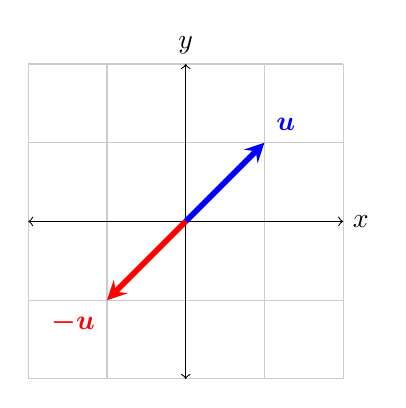
\begin{tikzpicture}
  \draw[thin,gray!40] (-2,-2) grid (2,2);
  \draw[<->] (-2,0)--(2,0) node[right]{$x$};
  \draw[<->] (0,-2)--(0,2) node[above]{$y$};
  \draw[line width=2pt,blue,-stealth](0,0)--(1,1)
        node[anchor=south west]{$\boldsymbol{u}$};
  \draw[line width=2pt,red,-stealth](0,0)--(-1,-1)
        node[anchor=north east]{$\boldsymbol{-u}$};
\end{tikzpicture}
\end{center}
\caption{\label{fig:vectors} Text size inside figure should be as big as
  caption's text. Text size inside figure should be as big as
  caption's text. Text size inside figure should be as big as
  caption's text. Text size inside figure should be as big as
  caption's text. Text size inside figure should be as big as
  caption's text. }
\end{figure}
%% %---------------------------


Here's a typical reference to a floating figure:
Figure~\ref{fig:vectors}. Floats should usually be placed where latex
wants then. Figure\ref{fig:vectors} is centered, and has a caption
that instructs you to make sure that the size of the text within the
figures that you use is as big as (or bigger than) the size of the
text in the caption of the figures. Please do. Really.

In our case, we've explicitly drawn the figure inlined in latex, to
allow this tex file to cleanly compile. But usually, your figures will
reside in some file.pdf, and you'd include them in your document
with, say, \textbackslash{}includegraphics.

Lists are sometimes quite handy. If you want to itemize things, feel
free:
\noindent
The noindent at the start of this paragraph in its tex version makes
it clear that it's a continuation of the preceding paragraph, as
opposed to a new paragraph in its own right.

\section{Conclusion}

{\footnotesize 
\bibliographystyle{acm}
\bibliography{p1}
}

\end{document}
